% Created 2019-09-16 Mon 12:00
% Intended LaTeX compiler: pdflatex
\documentclass[10pt,t]{beamer}
\usepackage[utf8]{inputenc}
\usepackage[T1]{fontenc}
\usepackage{graphicx}
\usepackage{grffile}
\usepackage{longtable}
\usepackage{wrapfig}
\usepackage{rotating}
\usepackage{amsmath}
\usepackage{textcomp}
\usepackage{amssymb}
\usepackage{capt-of}
\usepackage{hyperref}
\usetheme{default}
\author{L. Larrabee Strow}
\date{\today}
\title{\large TITLE}
\subtitle{\footnotesize{AIRS Science Team Meeting}}
\date{\vspace{0.1in}\footnotesize{October 3, 2018 \vfill}}
\author{L. Larrabee Strow\inst{1,2}, Sergio DeSouza--Machado\inst{1,2}, Steven Leroy\inst{3}, Howard Motteler\inst{2}, Chris Hepplewhite\inst{2}, and Steven Buczkowski\inst{2}}
\institute[UMBC]{\inst{1} UMBC Physics Dept. \and \inst{2}UMBC JCET \and \inst{3} AER}
\input beamer_setup
\usetheme{metropolis}
\metroset{titleformat title=allcaps}
\renewcommand{\UrlFont}{\small\tt}
\renewcommand*{\UrlFont}{\footnotesize}
\tolerance=1000
\RequirePackage{fancyvrb}
\DefineVerbatimEnvironment{verbatim}{Verbatim}{fontsize=\footnotesize}
\begin{document}

\maketitle
\addtobeamertemplate{block begin}{
  \setlength{\parsep}{0pt}
  \setlength{\topsep}{3pt plus 2pt minus 2.5pt}
  \setlength{\itemsep}{0pt plus 0pt minus 2pt}
  \setlength{\partopsep}{2pt}
}

\begin{frame}[label={sec:orgd23692c}]{SAMPLE: Motivation}
\begin{itemize}
\item Produce Level 1b CHIRP radiances for retrievals
\item Produce Level 3 climate-level gridded CHIRP radiance products
\item Goals
\begin{itemize}
\item Minimize sensitivity to a-priori estimates, etc.
\item Remove artificial sampling biases
\item Perform as much analysis in radiance space for error traceability
\end{itemize}
\item Geophysical Products
\begin{itemize}
\item Level 3 T/Q anomalies and trends (and surface T?)
\end{itemize}
\end{itemize}
\vspace{0.05in}

This approach is in principle very simple and quick.  Allows frequency re-processing. 

\vspace{0.05in}

What's Hard: 
\begin{itemize}
\item Dealing with clouds
\item AIRS radiometric stability estimates (ie. how good?)
\end{itemize}
\end{frame}

\begin{frame}[label={sec:org91507c7}]{SAMPLE 2x Figs}
\vspace{-0.3in}

\begin{columns}
\begin{column}{0.55\columnwidth}
\begin{block}{\footnotesize Some Small Title}
\vspace{-0.1in}
\begin{center}
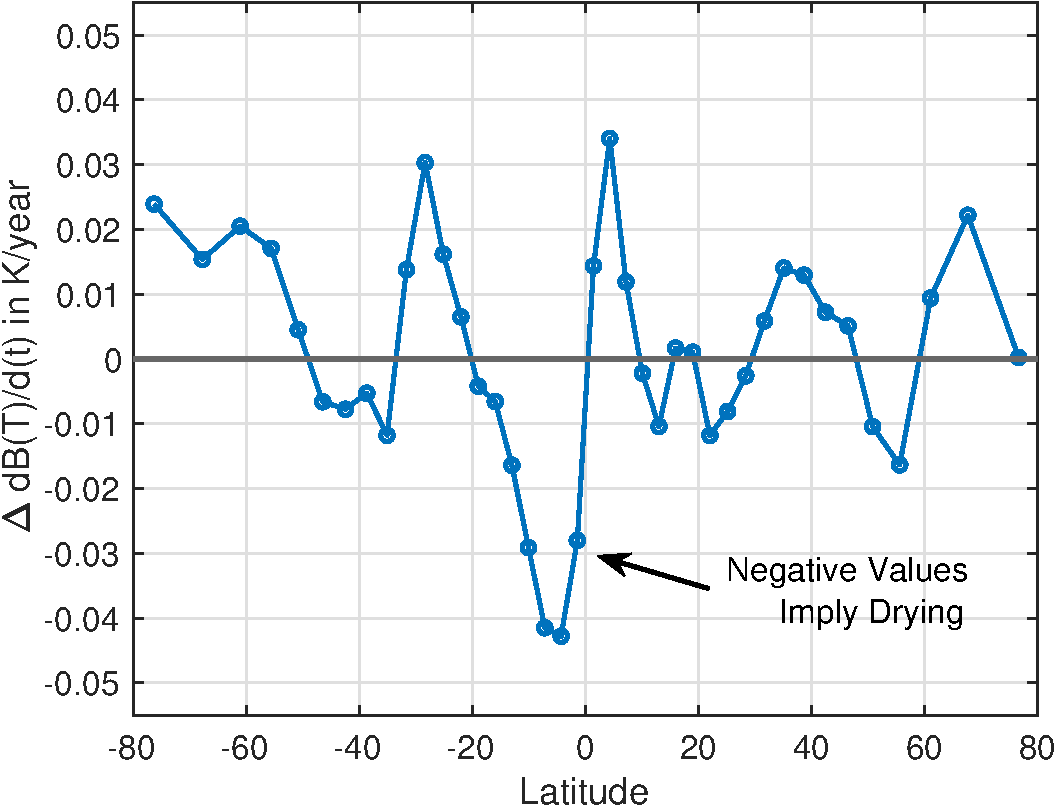
\includegraphics[width=\linewidth]{./Figs/Pdf/drying_in_convective_regions_v2.pdf}
\end{center}

\footnotesize
AIRS, CrIS, IASI are \emph{all} very stable\\
CLARREO has removed us from this figure!
\end{block}
\end{column}

\begin{column}{0.55\columnwidth}
\begin{block}{\footnotesize Another Small Title}
\vspace{-0.1in}
\begin{center}
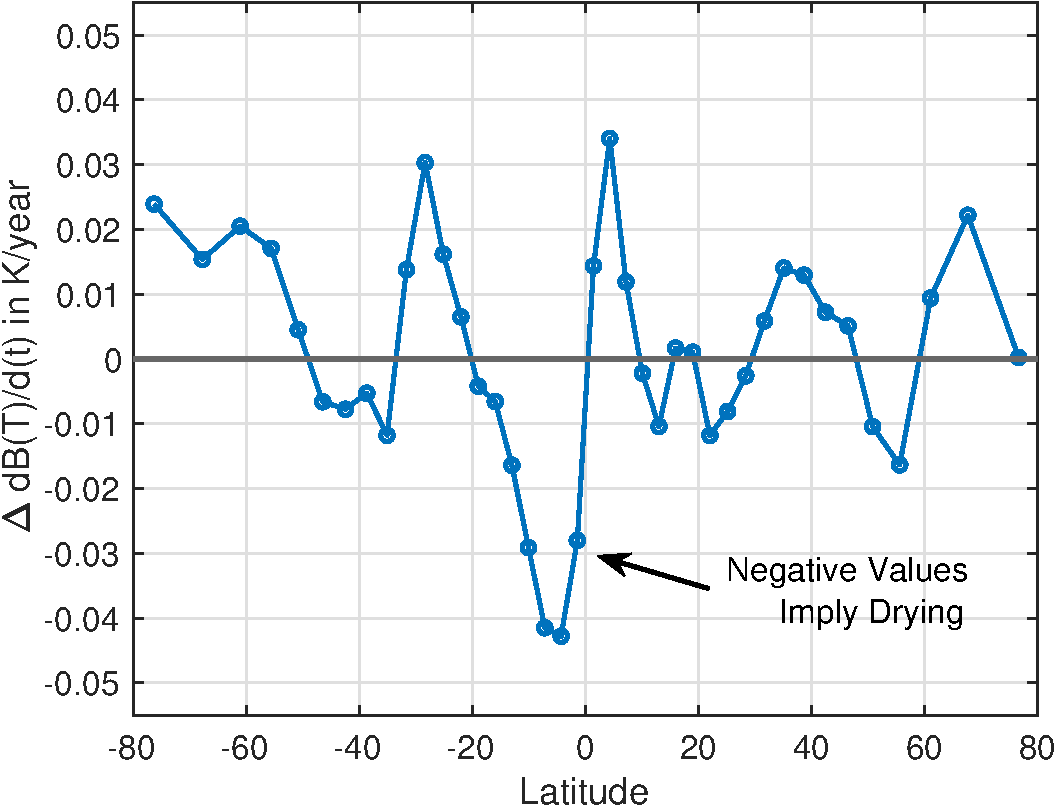
\includegraphics[width=\linewidth]{./Figs/Pdf/drying_in_convective_regions_v2.pdf}
\end{center}

\footnotesize
These are 2-\(\sigma\) B(T) statistical uncertainties due to inter-annual variability.  

Some channels, some latitudes not gaussian (strat sudden warmings, QBO, etc.)
\end{block}
\end{column}
\end{columns}
\end{frame}



\begin{frame}[label={sec:orgd2a29c0}]{SAMPLE 4x Figs}
\vspace{-0.35in}

\begin{columns}
\begin{column}{0.45\columnwidth}
\begin{block}{\footnotesize Some Small Title}
\vspace{-0.1in}
\begin{center}
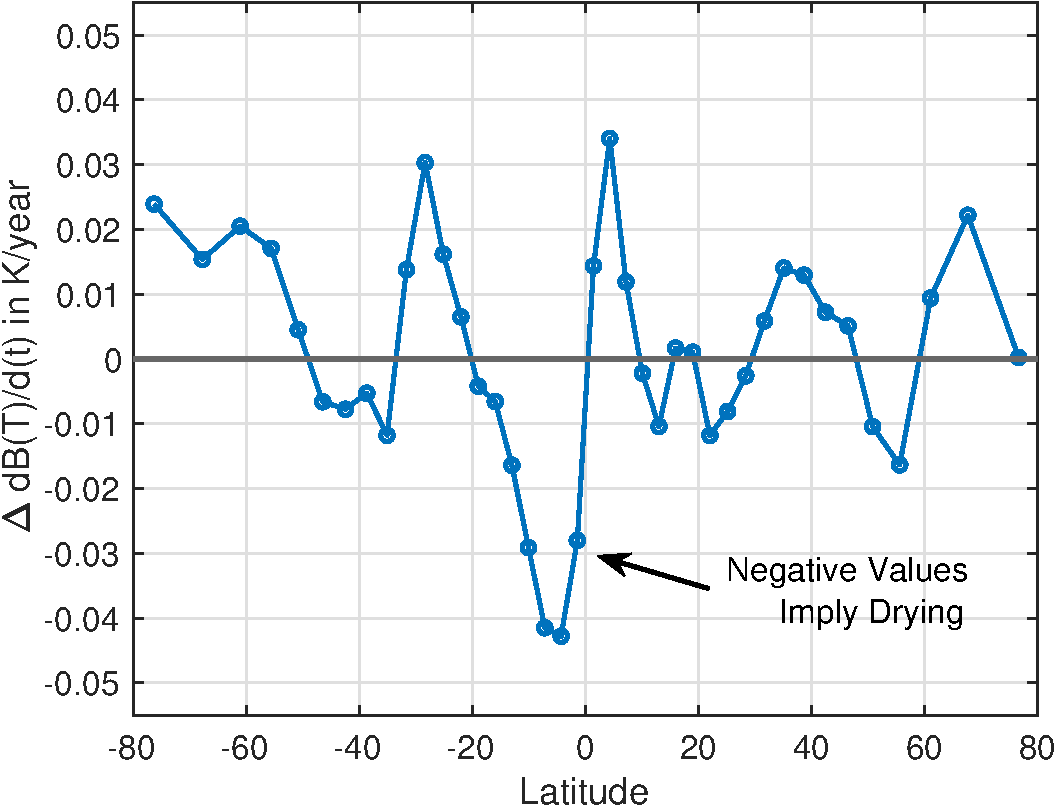
\includegraphics[width=\linewidth]{./Figs/Pdf/drying_in_convective_regions_v2.pdf}
\end{center}
\end{block}
\end{column}

\begin{column}{0.45\columnwidth}
\begin{block}{\footnotesize Another Small Title}
\vspace{-0.1in}
\begin{center}
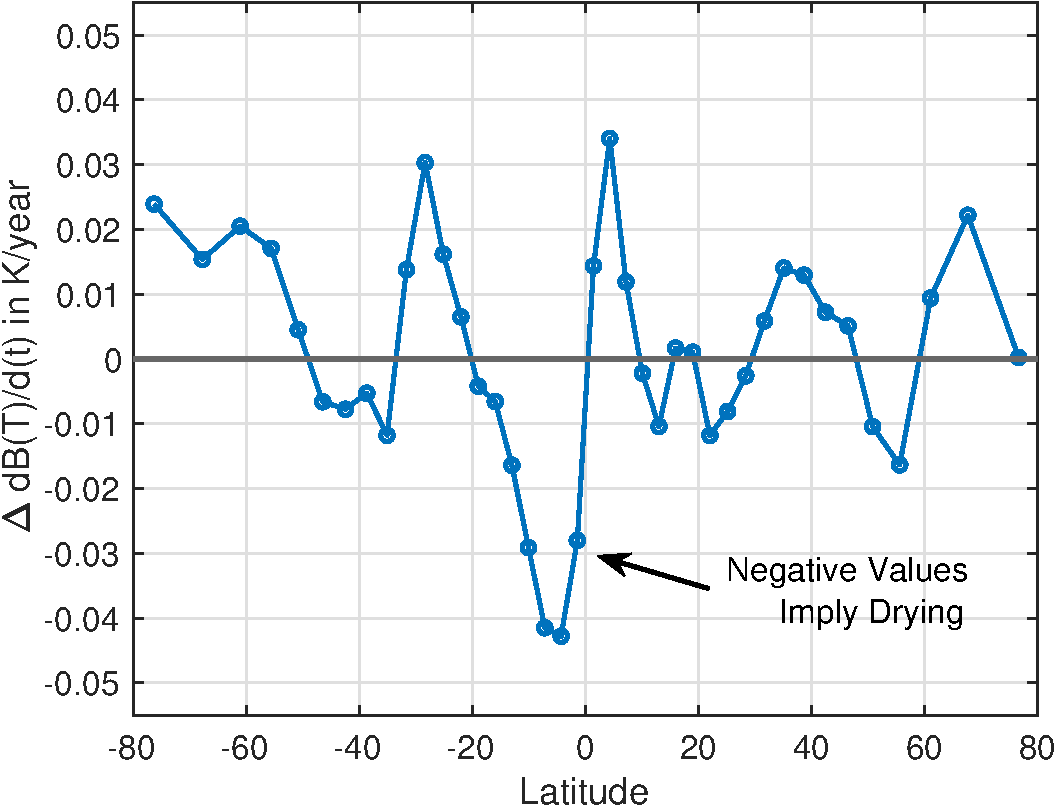
\includegraphics[width=\linewidth]{./Figs/Pdf/drying_in_convective_regions_v2.pdf}
\end{center}
\end{block}
\end{column}
\end{columns}

\vspace{-0.25in}

\begin{columns}
\begin{column}{0.45\columnwidth}
\begin{block}{\footnotesize Some Small Title}
\vspace{-0.1in}
\begin{center}
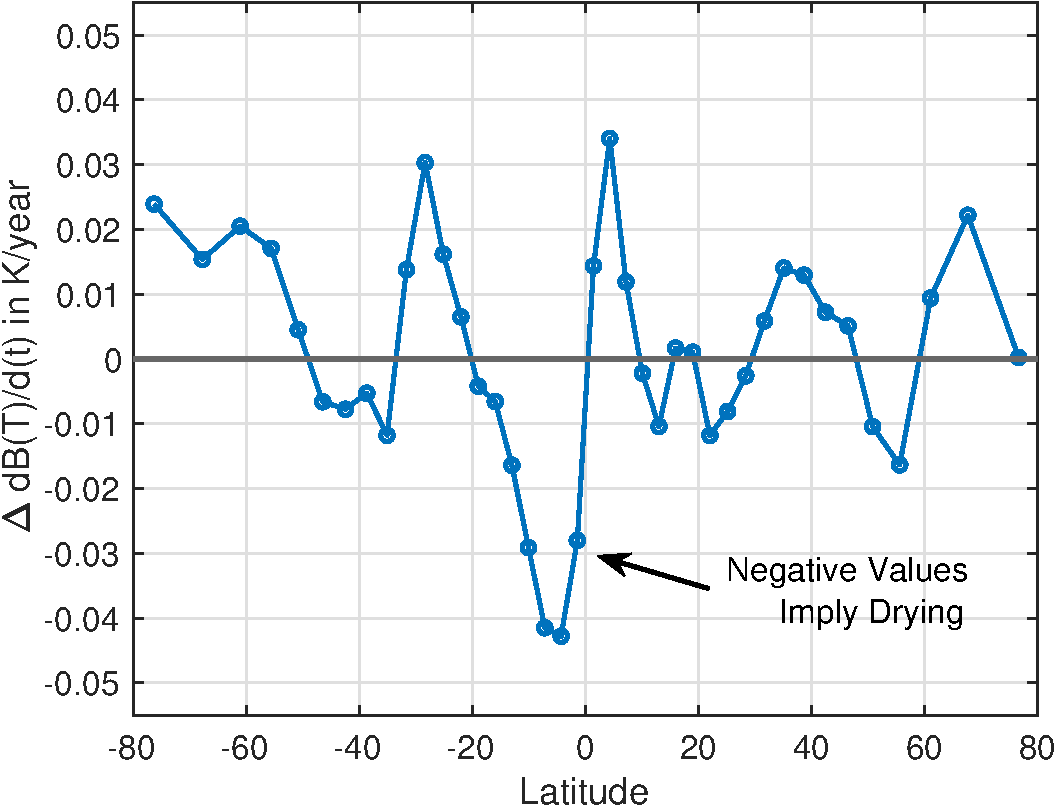
\includegraphics[width=\linewidth]{./Figs/Pdf/drying_in_convective_regions_v2.pdf}
\end{center}
\end{block}
\end{column}

\begin{column}{0.45\columnwidth}
\begin{block}{\footnotesize Another Small Title}
\vspace{-0.1in}
\begin{center}
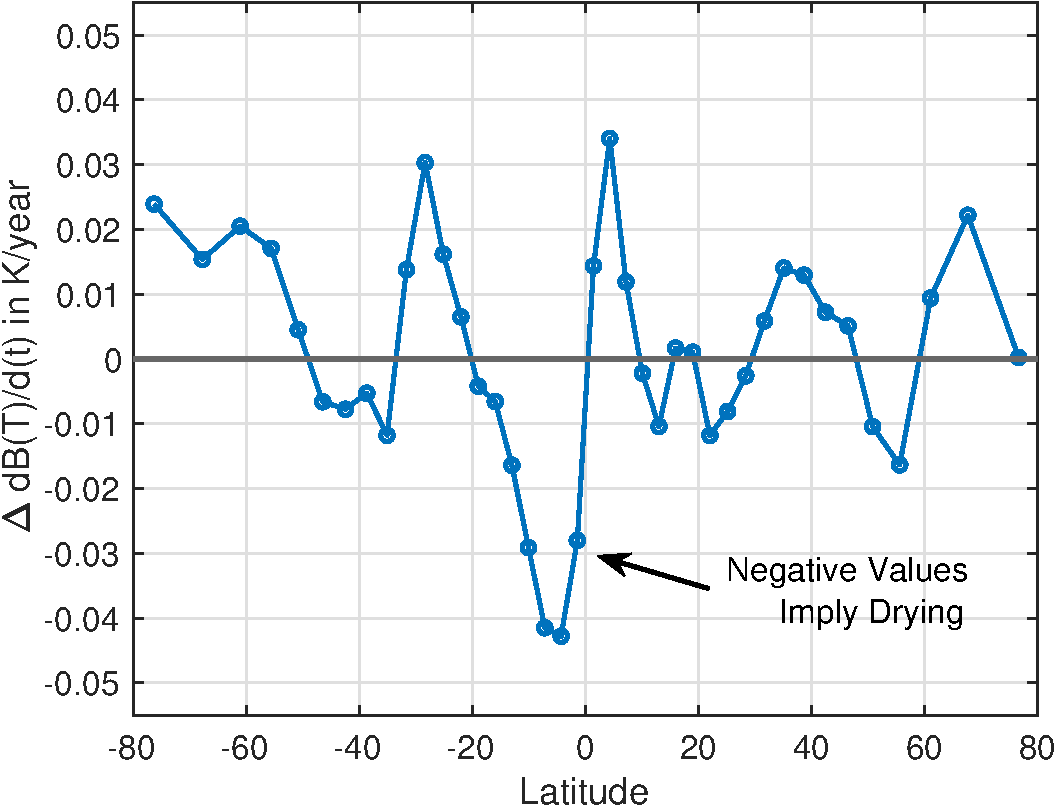
\includegraphics[width=\linewidth]{./Figs/Pdf/drying_in_convective_regions_v2.pdf}
\end{center}
\end{block}
\end{column}
\end{columns}
\end{frame}
\end{document}